% Indicate the main file. Must go at the beginning of the file.
% !TEX root = ../main.tex

%%%%%%%%%%%%%%%%%%%%%%%%%%%%%%%%%%%%%%%%%%%%%%%%%%%%%%%%%%%%%%%%%%%%%%%%%%%%%%%%
% 03_results
%%%%%%%%%%%%%%%%%%%%%%%%%%%%%%%%%%%%%%%%%%%%%%%%%%%%%%%%%%%%%%%%%%%%%%%%%%%%%%%%


\section{Results}
\label{results}

\subsection{Different Label Types}%%%%%%%%%%%%%%%%%%%%%%%%%%%%%%%%%%%%%%%%%%%%%%


\subsection{Augmentation}%%%%%%%%%%%%%%%%%%%%%%%%%%%%%%%%%%%%%%%%%%%%%%%%%%%%%%%


\subsection{Hyperparameter Tuning}%%%%%%%%%%%%%%%%%%%%%%%%%%%%%%%%%%%%%%%%%%%%%%

\begin{figure}[H]
    \centering
    \captionsetup{width=0.8\linewidth}
    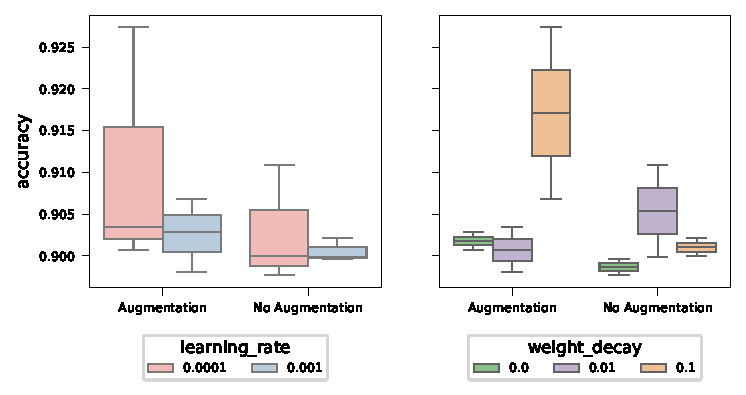
\includegraphics{figures/hp_tuning_boxplot.pdf}
    \caption{Accuracy of the models for the different hyperparameter grouped by use of data augmentation.}
    \label{fig:hp_tuning_boxplot}
\end{figure}



\subsection{Best Model}%%%%%%%%%%%%%%%%%%%%%%%%%%%%%%%%%%%%%%%%%%%%%%%%%%%%%%%%%

The best performing model was the one for the simplified perviousness classification
with the following hyperparameter:
\begin{itemize}
    \item Learning rate: 0.001
    \item Weight decay: 0.01
    \item Data augmentation applied
\end{itemize}
It achieved an accuracy of 0.927 and a weighted F1 Score of 0.927.
The F1 Score per class was 0.92 for class 'unsealed' and 0.93 for class 'sealed'.
For a visual inspection of the predictions refer to \autoref{fig:best_model_visual}.

\begin{figure}[H]
    \centering
    \captionsetup{width=0.8\linewidth}
    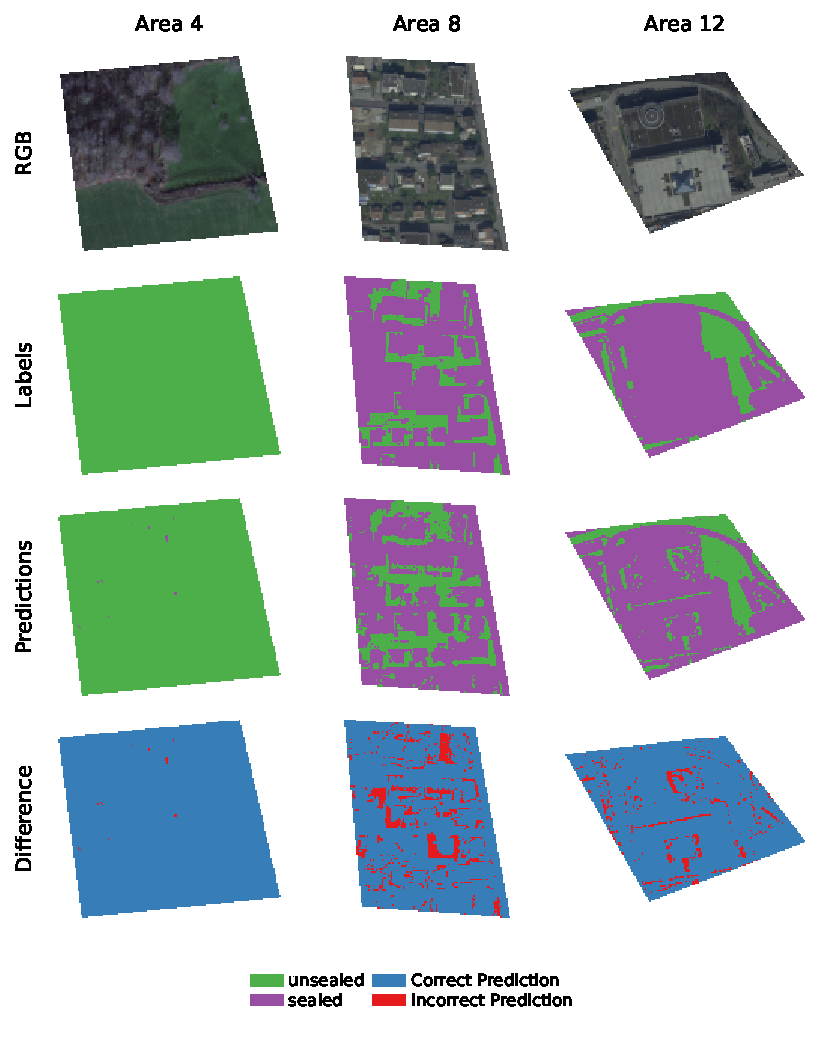
\includegraphics{figures/best_model_visual.pdf}
    \caption{Visual inspection of the predictions for the test areas of the best model.}
    \label{fig:best_model_visual}
\end{figure}